\chapter{Design}

\section{Architecture overview}

The Connectivity Manager is logically located between the EMM and the cloud infrastructure and provides the following two functionalities:
\begin{itemize}
\item \textbf{Optimal Instance Placement:} During the deployment of a stack an algorithm chooses where individual instances are placed within the cloud infrastructure.
\item \textbf{Service-Level-Agreement enforcement:} Depending on the services that an instance provides to the rest of the stack, certain requirements for its network performance need to be fulfilled.
\end{itemize}

\begin{figure}[H]
\centering

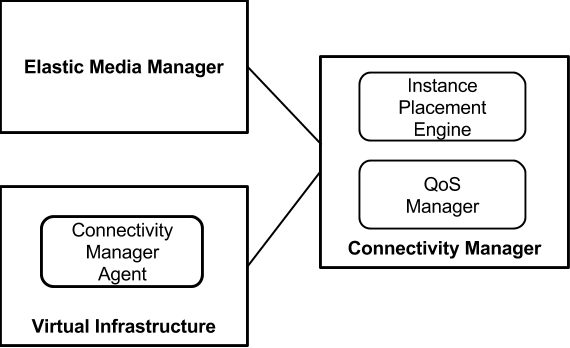
\includegraphics[width=0.5\textwidth]{images/design/functional_architecture}

\caption{High-level architecture of the Connectivity Manager}
\end{figure}

The \textit{Instance Placement Engine} determines if and where the instances should be deployed. It does so by comparing the current utilization and capacity of the available compute nodes within the availability zone.

The \textit{QoS Manager} enforces different QoS policies based on the type of service that the instance is grouped in. A guaranteed and maximum bit-rate for the network port of an instance can be set. This way a certain network performance can be insured.

\section{Connection between Manager \& Agent}

The Connectivity Manager and Agent are two separate applications that communicate using a ReST API. 

\begin{figure}[H]
\centering

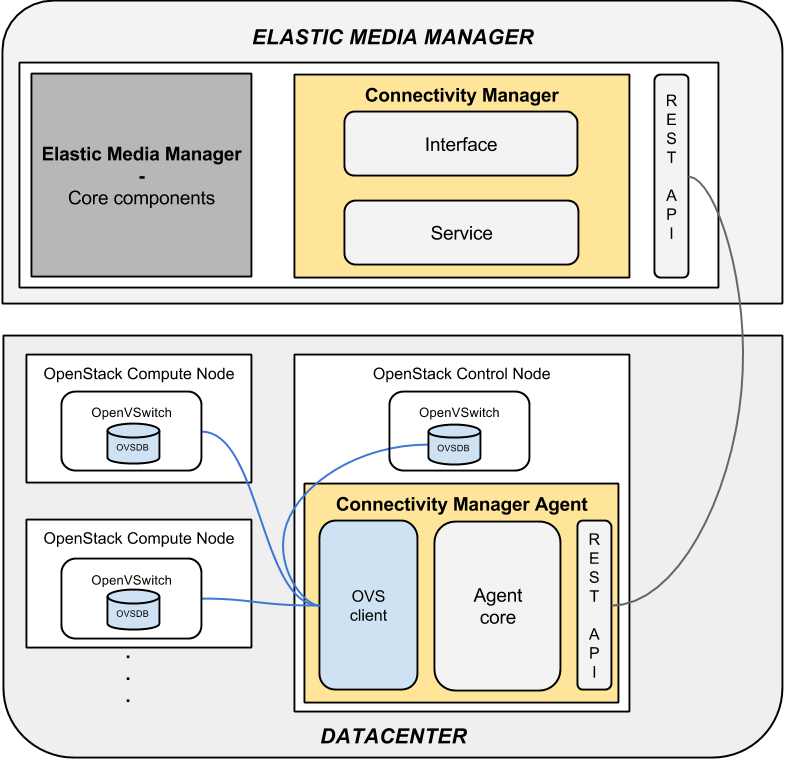
\includegraphics[width=0.6\textwidth]{images/design/modular_architecture_cm_cma}

\caption{Minimized architecture of the Connectivity Manager and its integrations}
\end{figure}

This design was chosen first of all because the Connectivity Manager is integrated in the EMM, which is required to be placed anywhere outside of the data center. Second of all the Connectivity Manager Agent needs to  the OVSDB on the compute nodes and consequently needs to be within the internal management network of the OpenStack infrastructure.

The sequence diagram below displays the work-flow that the CM passes during the run-time.

\begin{figure}[H]
\centering

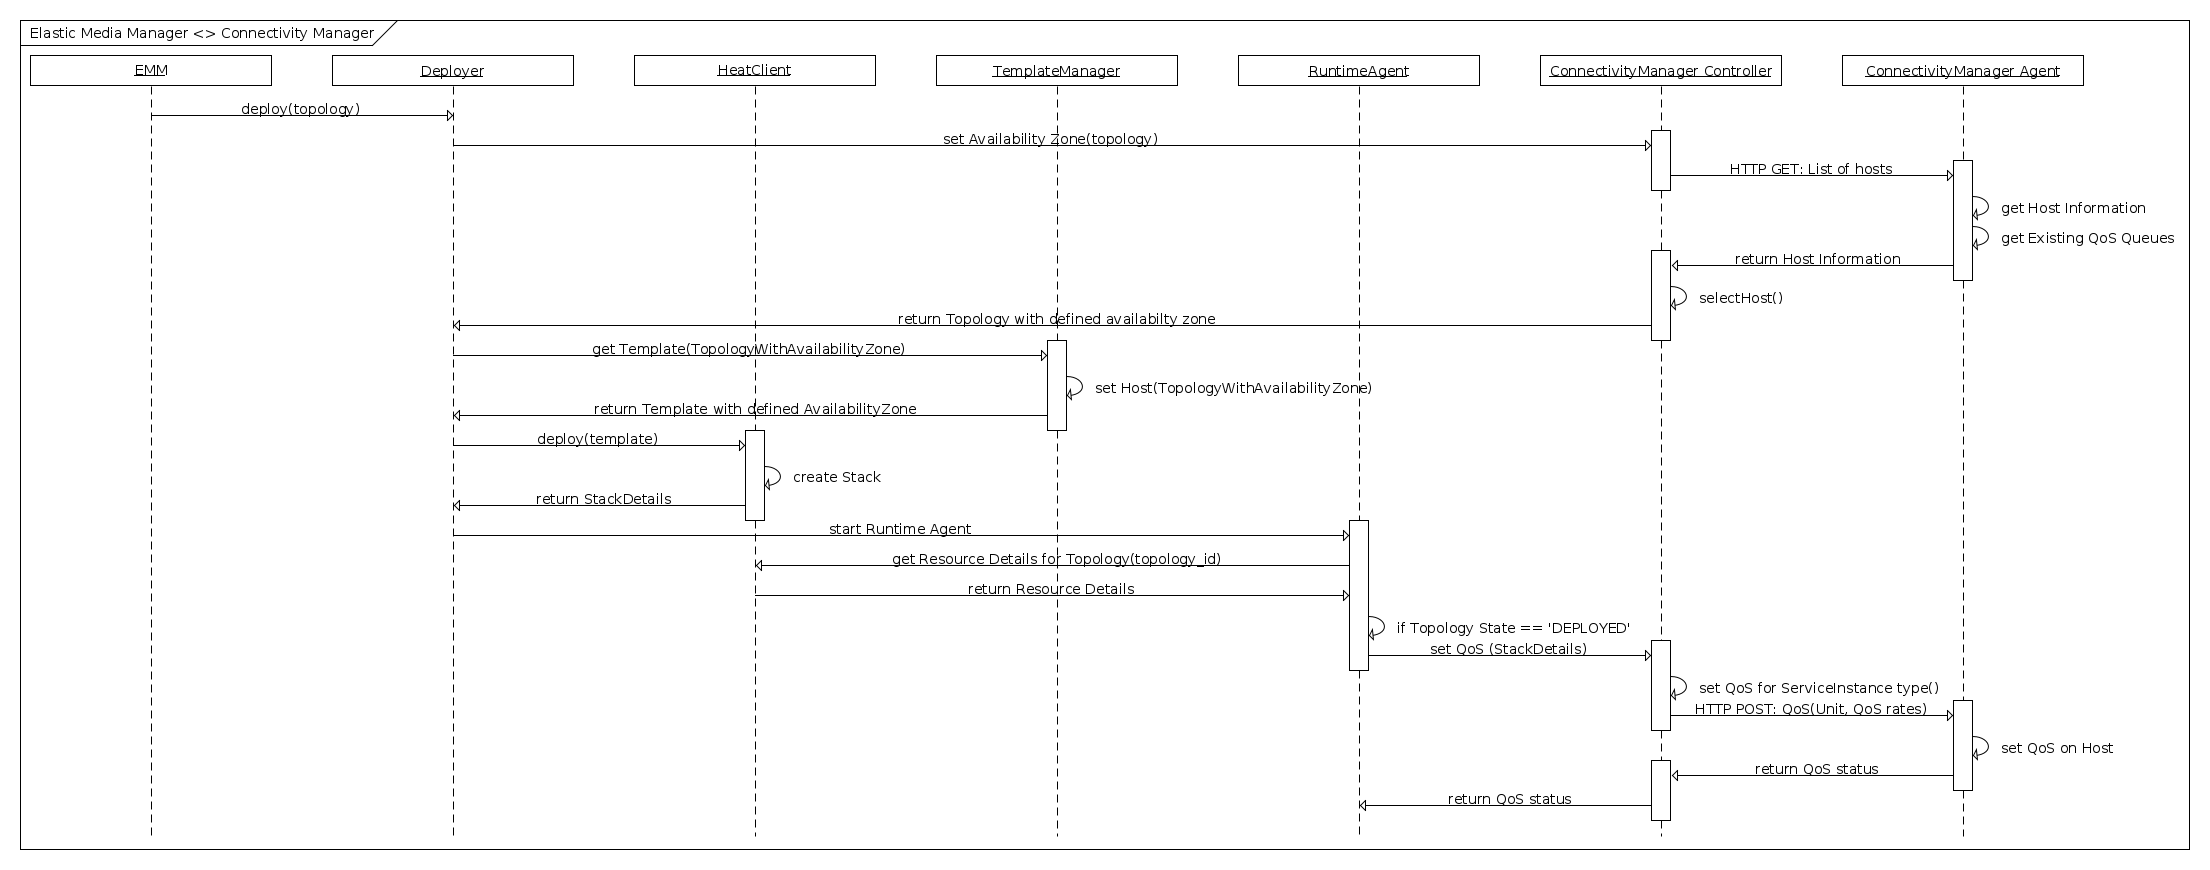
\includegraphics[width=0.9\textwidth]{images/design/sequence_diagram}

\caption{Workflow: Deployment of stack \& Assignment of QoS policies}
\end{figure}

As can be seen, the Connectivity Manager receives the Topology that contains a description of the configuration and specifications of the whole cloud. For the placement decision the CM to needs to get the information about the current state of the infrastructure. This exchange with the CM Agent occurs through the given API. Upon reception of that data, the placement algorithm sets the availability zone for each instance within the topology. The topology is then converted into a Heat template by the Template Manager. Once the template got deployed by the Heat Client a runtime agent starts. The purpose of the runtime agent is to continuously check the state of the stack. Once the stack has reached the 'DEPLOYED' state, the runtime agent requests the CM to set the QoS policies according to previously configured values. This configuration is subsequently transmitted to the CM Agent whose task is then to enable it on the according ports of the instances within the Open vSwitch.

\section{Design of Connectivity Manager}


\begin{figure}[H]
\centering

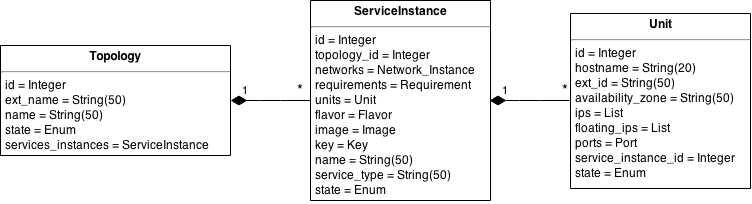
\includegraphics[width=0.9\textwidth]{images/design/cm_topology_object}

\caption{Deployment: Topology object from EMM}
\end{figure}


\subsection{Algorithm for Instance Placement}



\newpage
\section{Design of Connectivity Manager Agent}

\begin{figure}[H]
\centering

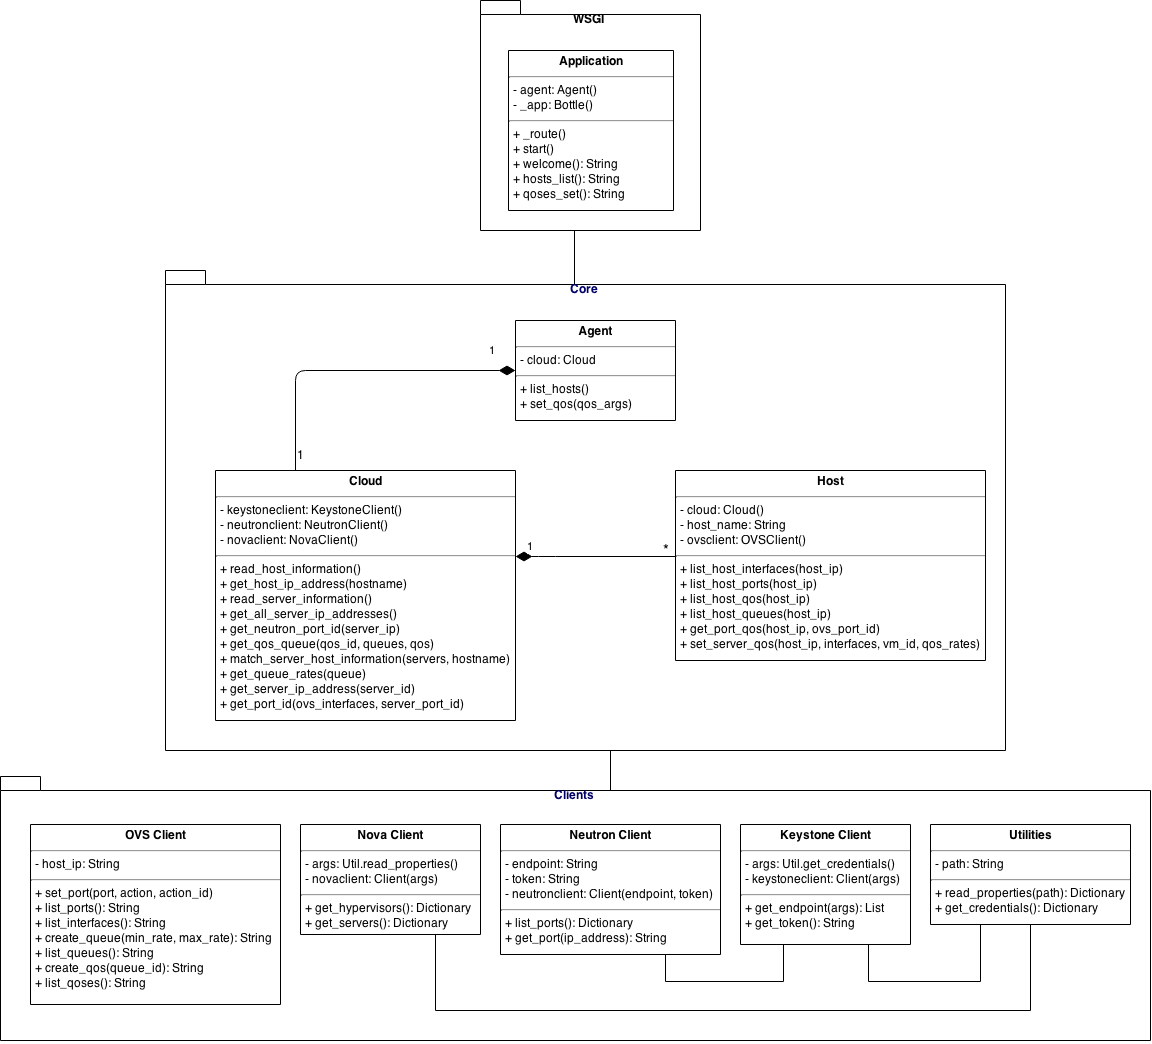
\includegraphics[width=0.7\textwidth]{images/design/cm_agent_class_diagram}

\caption{Class diagram: Connectivity Manager Agent - Core package}
\end{figure}


\begin{figure}[H]
\centering

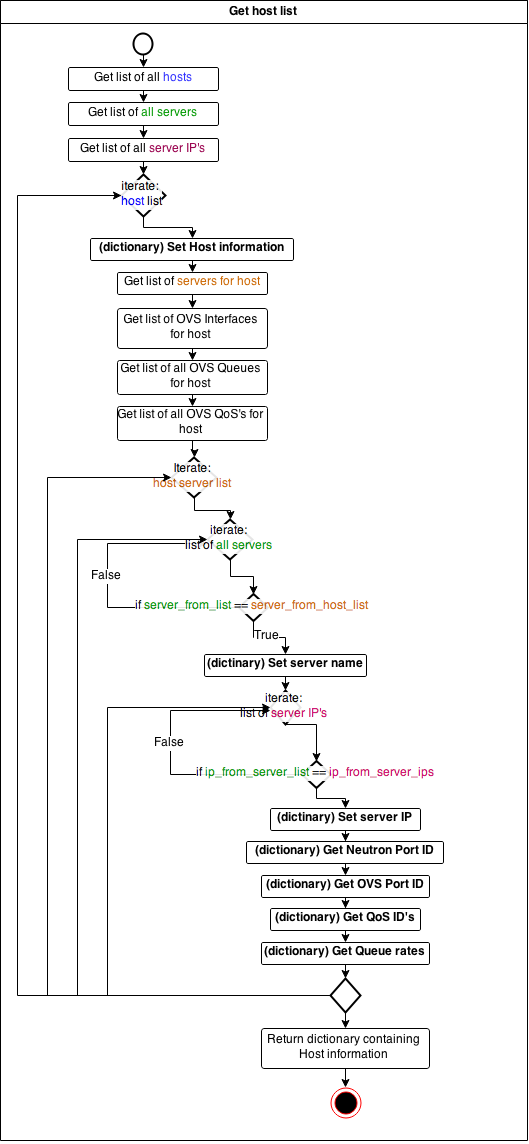
\includegraphics[width=0.7\textwidth]{images/design/activity_host_list}

\caption{Activity diagram: Get list of hosts}
\end{figure}

\begin{figure}[H]
\centering

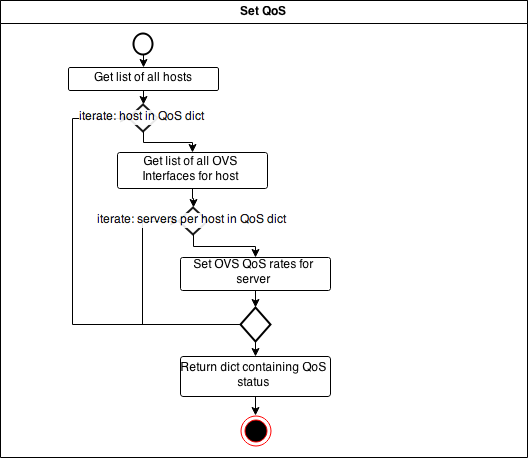
\includegraphics[width=0.7\textwidth]{images/design/activity_set_qos}

\caption{Activity diagram: Set QoS rates for all servers}
\end{figure}

\begin{figure}[H]
\centering

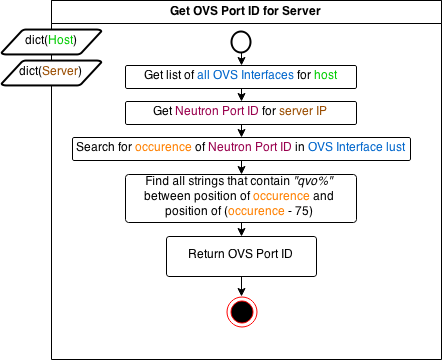
\includegraphics[width=0.7\textwidth]{images/design/activity_get_ovs_port_server}

\caption{Activity diagram: Get OVS Port ID for server}
\end{figure}

\begin{figure}[H]
\centering

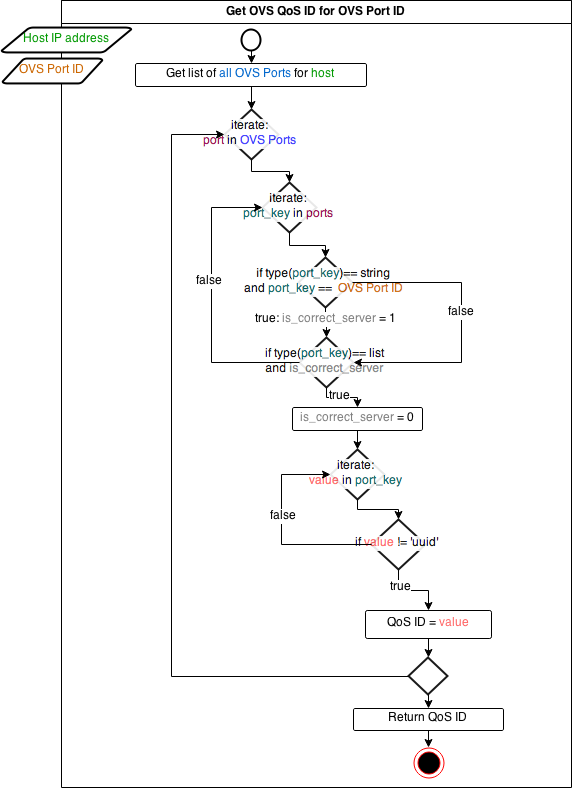
\includegraphics[width=0.7\textwidth]{images/design/activity_get_qos_id_for_ovs_port}

\caption{Activity diagram: Get QoS ID for OVS Port}
\end{figure}





\section{Conclusion}